\section{Metodo delle tangenti}
Fino ad ora abbiamo scelto come funzione $g$ per il metodo iterativo qualcosa nella forma
\[ g(x) = x - f(x) \]
Per il metodo che vedremo tra poco scegliamo invece $g$ nella forma
\[ g(x) = x - \frac{f(x)}{h(x)} \]
Dove $h(x)$ ricordiamo essere una funzione definita sugli \emph{zeri} di $f$. Il metodo che vediamo è chiamato
\textbf{metodo delle tangenti} o \textbf{metodo di Newton} e prende $h(x) = f'(x)$ definendo $g(x)$ come segue
\[ g(x) = x - \frac{f(x)}{f'(x)} \]
Otteniamo quindi il seguente metodo iterativo
\[ x_{k+1} = x_k - \frac{f(x_k)}{f'(x_k)} \]
Supponiamo di avere una funzione $f$ e di voler trovare $\alpha$ tale che $f(\alpha) = 0$. Supponiamo ora di
avere un punto $x_0$ e il valore della funzione calcolata in tale punto, ossia $f(x_0)$. Otteniamo così il
punto $(x_0, f(x_0)) \in f$.

Definiamo ora la retta tangente alla funzione passante per tale punto. L'equazione della tangente alla funzione
è la seguente
\[ y - f(x_0) = f'(x_0)(x - x_0) \]
Andiamo ora a calcolare l'intersezione della tangente con l'asse delle ascisse trovando così il nuovo punto $x_1$.
\[
	\begin{cases}
		y - f(x_0) = f'(x_0)(x_1 - x_0) \\
		y = 0
	\end{cases}
\]
Sostituendo $y = 0$ nella prima equazione otteniamo
\begin{align*}
	-f(x_0) =                 & f'(x_0)(x_1 - x_0)           \\
	-\frac{f(x_0)}{f'(x_0)} = & x_1 - x_0                    \\
	x_1 =                     & x_0 - \frac{f(x_0)}{f'(x_0)}
\end{align*}
Ecco che abbiamo ottenuto l'equazione di partenza del metodo. A questo punto non ci rimane che ripetere il
procedimento per $x_1$ fino a quando il metodo non converge.

La derivata di $g(x) = x - \frac{f(x)}{f'(x)}$, in questo caso, è la seguente
\[ g'(x) = 1 - \frac{f'(x) f'(x) - f''(x) f(x)}{f'(x)^2} = \frac{f''(x) f(x)}{f'(x)^2} \]
Se valutiamo $g'$ in $\alpha$ otteniamo
\[ g'(\alpha) = \frac{f''(\alpha) f(\alpha)}{f'(\alpha)^2} \]
Teniamo a mente però che $\alpha$ è radice della funzione $f$ e quindi vale
\[ f(\alpha) = 0 \quad \Rightarrow \quad g'(\alpha) = 0 < 1 \]
se $f'(\alpha) \neq 0$.Dunque, sotto quest'ipotesi, il metodo converge localmente.

\begin{example}
	Proviamo ora a calcolare la radice $\alpha$ dell'equazione
	\[ f(x) = e^{-x} - x = 0 \]
	con il metodo delle tangenti. Calcoliamo la derivata prima
	\[ f'(x) = -e^{-x} - 1 \]
	Supponiamo di scegliere $x_0 = 0$ e valutiamo la funzione in $x_0$, ottenendo il punto $(0, 1)$ da cui
	iniziare a iterare. La tangente $t_0$ alla funzione nel punto trovato ha equazione
	\[ y = -2x + 1 \]
	Calcoliamo quindi il punto $x_1$ ponendo $y=0$ e otteniamo $x_1 = \frac{1}{2}$
	Se adesso ripetiamo il procedimento otteniamo la tangente $t_1$ della funzione nel punto
	$(x_1, f(x_1)) = \left( \frac{1}{2}, \frac{1}{\sqrt{e}} - \frac{1}{2} \right)$, ossia
	\[ y = - x \left( \frac{1}{\sqrt{e}} + 1 \right) + \frac{3}{2 \sqrt{e}} \]
	\begin{center}
		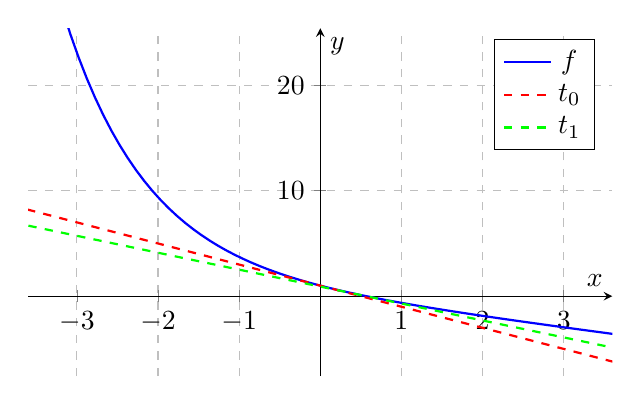
\begin{tikzpicture}
			\begin{axis}[
					font=\normalsize,
					width=9cm,
					height=6cm,
					axis lines = center,
					xlabel = $x$,
					ylabel = $y$,
					xmin = -3, xmax = 3,
					grid = both,
					grid style = dashed,
					legend pos = north east,
					enlargelimits
				]

				\addplot [ samples=100, thick, color=blue ] {exp(-x) - x};

				\addplot [ thick, dashed, color=red] {-2 * x + 1};

				\addplot [thick, dashed, color=green] { - 1.606 * x + 0.909 };

				\legend{ $f$, $t_0$, $t_1$ }
			\end{axis}
		\end{tikzpicture}
	\end{center}
	Come possiamo vedere, la seconda tangente (in verde) incontra l'asse delle ascisse in un punto più vicino ad
	$\alpha$.
\end{example}

Nel caso in cui $f'(\alpha) = 0$ il metodo converge comunque anche se non possiamo dire di avere convergenza
locale.

\begin{example}
	Consideriamo ora l'equazione
	\[ f(x) = x^2 = 0 \]
	Vediamo facilmente che l'equazione ha due radici reali coincidenti $\alpha = \beta = 0$. La derivata prima
	equivale però a
	\[ f'(x) = 2x \]
	e quindi $f'(0) = 0$. Andiamo però ad analizzare la successione generata dal metodo delle tangenti.
	\[ x_{k+1} = x_k - \frac{x_k^2}{2 x_k} = x_k - \frac{x_k}{2} = \frac{x_k}{2} \]
	Ogni elemento della successione è la metà del precedente e quindi l'elemento al passo $(k+1)$-esimo equivale a
	\[ x_{k+1} = \frac{x_0}{2^k} \]
	Ed è facile notare che
	\[ \lim_{k \to +\infty} \frac{x_0}{2^k} = 0 \]
	qualsiasi sia $x_0$, dunque il metodo è convergente.
\end{example}

\subsection{Convergenza locale}
Il metodo delle tangenti è ad oggi uno degli algoritmi di scelta. Il primo motivo è legato ad una condizione di
convergenza locale anche sotto ipotesi molto generali.

\begin{theorem}
	Sia $f : [a, b] \to \R$, $f \in C^2([a, b])$ e sia $\alpha \in (a, b)$ tale che
	\[ f(\alpha) = 0 \quad \wedge \quad f'(\alpha) \neq 0 \]
	allora esiste
	\[ I_\alpha = [\alpha - \rho, \alpha + \rho] \subseteq [a, b] \]
	tale che ogni $x_0 \in I_\alpha$ soddisfa queste due proprietà
	\[ x_k \in I_\alpha \quad \wedge \quad \lim_{k \to +\infty} x_k = \alpha \]
	\begin{proof}
		Dato che $f$ è una funzione continua con derivata prima continua possiamo dire che esiste un intorno di
		$\alpha$ che chiamiamo $\hat{I}_\alpha$ tale che $f'(x) \neq 0$ per ogni $x \in \hat{I}_\alpha$. Questo
		ci permette di definire in $\hat{I}_\alpha$ la funzione $g : \hat{I}_\alpha \to \R$
		\[ g(x) = x - \frac{f(x)}{f'(x)} \]
		Dato che $x$, $f(x)$ e $f'(x)$ sono continue e $f'(x) \neq 0$ allora possiamo dire che $g(x)$ è una
		funzione continua con derivata prima
		\[ g'(x) = \frac{f(x) f''(x)}{f'(x)^2} \]
		Come abbiamo detto all'inizio $f \in C^2([a, b])$ e $f'(x) \neq 0$ quindi $g \in C^1(\hat{I}_\alpha)$.
		Possiamo ora valutare $g'(\alpha)$ che vale
		\[ g'(\alpha) = \frac{f(\alpha) f''(\alpha)}{f'(\alpha)^2} \]
		Sappiamo che $\alpha$ è uno zero di $f$ e che $f'(x) \neq 0$, quindi $g'(\alpha) = 0$. Dunque per il
		corollario \ref{coro: punto_fisso} possiamo dire che $\alpha$ è un punto \emph{attrattivo} ed esiste
		$I_\alpha \subseteq \hat{I}_\alpha$ tale che valgono le proprietà
		\[ x_k \in I_\alpha \quad \wedge \quad \lim_{k \to +\infty} x_k = \alpha \]
		Questo teorema ci dice che $f'(x) \neq 0$ è condizione sufficiente affinché ci sia convergenza locale.
	\end{proof}
\end{theorem}

\subsection{Velocità di convergenza}
Prima di parlare della velocità di convergenza del metodo delle tangenti chiariamo meglio il concetto di
\textbf{velocità di convergenza}. Supponiamo di avere una successione $x_k \to \alpha$ e che $x_k \neq \alpha$
per ogni $k$. Allora possiamo dire che
\begin{itemize}
	\item La successione converge \textbf{linearmente} se
	      \[ \lim_{k \to +\infty} \frac{|x_{k+1} - \alpha|}{|x_k - \alpha|} = L \]
	      con $0 < L < 1$.
	\item Si ha una convergenza \textbf{almeno quadratica} se
	      \[ \lim_{k \to +\infty} \frac{|x_{k+1} - \alpha|}{|x_k - \alpha|^2} = L \]
	      con $L \in \R$.
\end{itemize}

\paragraph{Convergenza lineare}
Nel primo caso il valore di $L$ ci fornisce il rapporto tra l'errore al passo $k+1$ e quello al passo $k$. Questo
si traduce in una riduzione dell'errore ad ogni passo, di un fattore $L$.

Se $L$ ha valore molto vicino a $1$ significa che il metodo converge lentamente dato che la differenza tra i due
sarà minima. Al contrario se $L \to 0$ la differenza tra i due errori è grande e il metodo converge più
velocemente.

\paragraph{Convergenza almeno quadratica}
Se abbiamo questo tipo di convergenza possiamo dire l'errore al passo $k$ è circa il quadrato dell'errore al passo
$k+1$. Si può dimostrare che il metodo delle tangenti ha un tipo di convergenza almeno quadratica.

\subsection{Convergenza in largo}
Per ora siamo solo in grado di dire che, sotto opportune ipotesi, esiste un intorno della soluzione entro il quale
abbiamo convergenza locale per ogni punto iniziale. Non abbiamo però strumenti per determinare l'ampiezza di
tale intorno e quindi non abbiamo la certezza che il punto iniziale scelto inneschi la convergenza locale.

\begin{theorem}[Convergenza in largo]\label{th: convergenza_largo}
	Sia $f : [a, b] \to \R$, $f \in C^2([a, b])$ e sia $\alpha \in (a, b)$ tale che $f(\alpha) = 0$. Se esiste
	\[ I_\alpha = (\alpha, \alpha + \delta] \subseteq [a, b] \]
	tale che
	\[ f(x) f''(x) > 0 \quad \wedge \quad f'(x) \neq 0 \]
	per ogni $x \in I_\alpha$ allora per ogni $x_0 \in I_\alpha$ vale
	\[ \lim_{k \to +\infty} x_k = \alpha \]
\end{theorem}

\paragraph{Intervallo destro}
Di questo teorema non facciamo la dimostrazione ma proviamo a capire meglio la situazione. Stiamo dunque cercando
di individuare un \textbf{intervallo destro} entro il quale valgono le ipotesi del teorema. Questo ci permette di
avere vincoli più deboli rispetto a prima, dove invece dovevamo cercare un intorno circolare di $\alpha$.

Consideriamo come primo caso la radice $\alpha$ dell'equazione $f(x) = 0$ e un certo $\delta$ tale che
nell'intervallo $(\alpha, \alpha + \delta]$ sono valide le ipotesi del teorema.

\paragraph{Derivata positiva} Supponiamo, più nello specifico, che $f' > 0$ nel suddetto intervallo. Dato che
$f' > 0$ e che $\alpha$ è uno zero di $f$ significa che, nell'intervallo appena definito, questa non cambia
segno ed è crescente.

Inoltre dato che in quell'intervallo $f$ è positiva anche $f'' > 0$ e dunque la funzione, in quell'intervallo è
convessa. Se ora proviamo a partire da un qualsiasi $x_0$ nell'intervallo avremo una successione
\textbf{monotona decrescente} che converge ad $\alpha$.

\paragraph{Derivata negativa} Se consideriamo il caso $f' < 0$ sullo stesso intervallo abbiamo che $f$ è negativa
decrescente nell'intervallo e anche $f'' < 0$ dunque la funzione è concava. Come prima possiamo partire da un
qualsiasi punto all'interno dell'intervallo e il metodo genera una successione \textbf{monotona decrescente} che
converge ad $\alpha$.

\paragraph{Intervallo sinistro}
In realtà il teorema si può estendere anche agli \textbf{intervalli sinistri}, ma in questo caso la successione
generata dal metodo sarà \textbf{monotona crescente}.

\begin{example}
	Supponiamo di voler determinare il numero di soluzioni reali dell'equazione
	\[ f(x) = e^x + x - 2 = 0 \]
	e di voler studiare la convergenza del metodo delle tangenti per l'approssimazione tali soluzioni.

	Partiamo col dire che $f \in C^\infty (\R)$ e che
	\[ \lim_{x \to +\infty} e^x + x - 2 = +\infty \quad \lim_{x \to -\infty} e^x + x - 2 = -\infty \]
	Calcoliamo ora derivata prima e seconda della funzione
	\[ f'(x) = e^x + 1 \quad f''(x) = e^x \]
	le quali sono sempre positive per ogni $x \in \R$. Possiamo ora tracciare il grafico approssimativo della
	funzione
	\begin{center}
		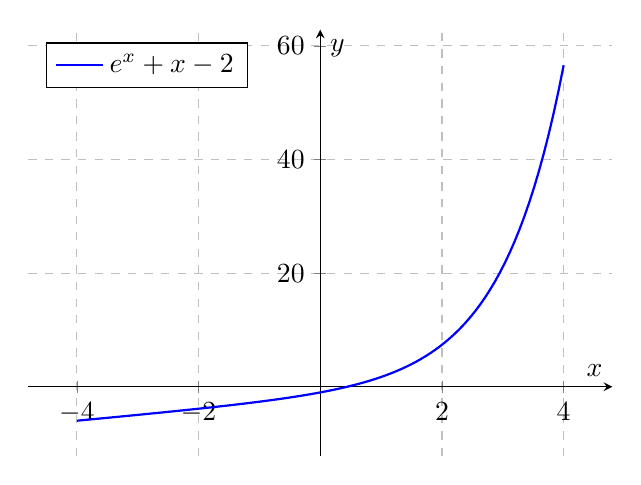
\begin{tikzpicture}
			\begin{axis}[
					font=\normalsize,
					width=9cm,
					height=7cm,
					axis lines = center,
					xlabel = $x$,
					ylabel = $y$,
					grid = both,
					grid style = dashed,
					legend pos = north west,
					enlargelimits
				]

				\addplot[
					domain=-4:4,
					thick,
					color=blue,
					samples=100
				] {exp(x) + x - 2};

				\legend{$e^x + x - 2$};
			\end{axis}
		\end{tikzpicture}
	\end{center}
	Ecco che possiamo quindi determinare che esiste ed è unica la soluzione reale $\alpha$ dell'equazione. Per
	localizzarla valutiamo
	\[ f(0) = -1 < 0 \quad f(1) = e - 1 > 0 \]
	quindi possiamo prendere come intervallo $(0, 1)$. Possiamo quindi dire che, in $\alpha$, il metodo è
	localmente convergente dato che $f \in C^\infty(\R)$ e $f'(\alpha) \neq 0$.

	Supponiamo ora di voler definire un intervallo entro il quale scegliere il punto inziale. Per farlo dobbiamo
	studiare la convergenza in largo. La funzione a destra di $\alpha$ è positiva crescente e convessa. Quindi
	le ipotesi del teorema \ref{th: convergenza_largo} (convergenza in largo) sono soddisfatte e possiamo
	affermare che per ogni $x_0 \geq \alpha$ il metodo converge ad $\alpha$.

	Proviamo a vedere cosa succede se prendiamo un punto iniziale $x_0 < \alpha$. In tal caso abbiamo che
	\begin{align*}
		x_1 - \alpha = & g(x_0) - g(\alpha)                               \\
		=              & g'(\xi) (x_0 - \alpha)                           \\
		=              & \frac{f(\xi) f''(\xi)}{f'(\xi)^2} (x_0 - \alpha)
	\end{align*}
	Studiamo il segno dei vari pezzi dell'ultima espressione. Per prima cosa possiamo dire che
	\[ x_0 - \alpha < 0 \]
	dato che $\alpha > 0$ e che siamo nell'ipotesi che $x_0 < \alpha$. La funzione a sinistra di $\alpha$ è
	negativa ma derivate prima e seconda sono sempre positive su tutto $\R$. Dunque possiamo affermare che
	\[ \frac{f(\xi) f''(\xi)}{f'(\xi)^2} < 0 \]
	Otteniamo quindi un prodotto tra due quantità negative, ne segue che
	\[ x_1 - \alpha > 0 \]
	In altre parole possiamo dire che possiamo prendere un qualsiasi $x_0 \in \R$, nel caso sia maggiore di
	$\alpha$ il metodo converge ad $\alpha$ normalmente, nel caso sia minore, il metodo, dopo un passo si sposta
	nell'intervallo destro di $\alpha$ e da lì inizia a convergere ad $\alpha$. Abbiamo quindi un caso di
	\textbf{convergenza globale}.
\end{example}
